
\documentclass[tikz,border=6pt]{standalone}
\usepackage{pgfplots}
\pgfplotsset{compat=1.18}
\usepgfplotslibrary{groupplots}
\definecolor{lineblue}{RGB}{43,120,186}
\definecolor{lineorange}{RGB}{243,156,18}
\begin{document}
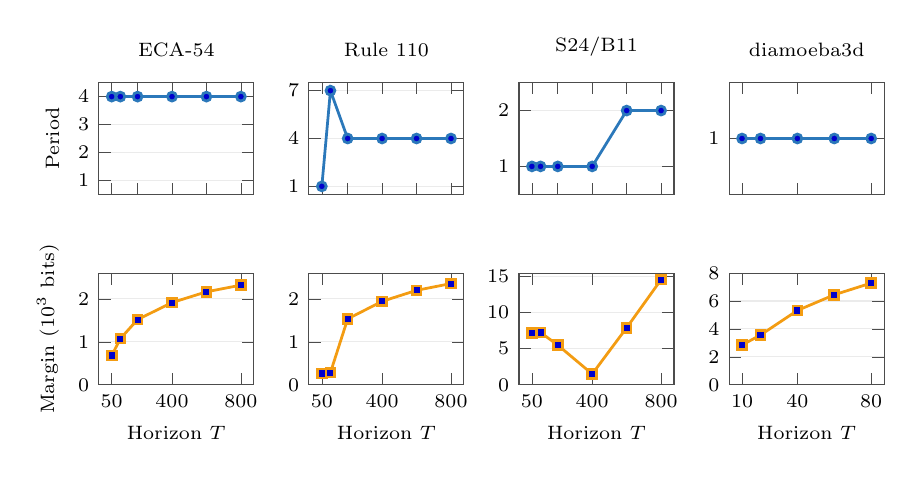
\begin{tikzpicture}
\begin{groupplot}[
  group style={group size=4 by 2, horizontal sep=7mm, vertical sep=10mm},
  width=3.55cm,
  height=3.0cm,
  axis line style={black!70},
  tick style={black!70},
  xticklabel style={font=\scriptsize},
  yticklabel style={font=\scriptsize},
  title style={font=\scriptsize, align=center},
  ylabel style={font=\scriptsize},
  xlabel style={font=\scriptsize},
  major grid style={draw=black!8},
  ymajorgrids=true,
  xmajorgrids=false
]
\nextgroupplot[title={ECA-54}, ymin=0.5, ymax=4.5, ytick={1,2,3,4}, ylabel={Period}, xticklabels={,,,,}, xtick={50,200,400,600,800}]
\addplot+[lineblue, mark=*, mark size=1.6pt, line width=1pt] coordinates {(50,4) (100,4) (200,4) (400,4) (600,4) (800,4)};

\nextgroupplot[title={Rule 110}, ymin=0.5, ymax=7.5, ytick={1,4,7}, xticklabels={,,,,}, xtick={50,200,400,600,800}]
\addplot+[lineblue, mark=*, mark size=1.6pt, line width=1pt] coordinates {(50,1) (100,7) (200,4) (400,4) (600,4) (800,4)};

\nextgroupplot[title={S24/B11}, ymin=0.5, ymax=2.5, ytick={1,2}, xticklabels={,,,,}, xtick={50,200,400,600,800}]
\addplot+[lineblue, mark=*, mark size=1.6pt, line width=1pt] coordinates {(50,1) (100,1) (200,1) (400,1) (600,2) (800,2)};

\nextgroupplot[title={diamoeba3d}, ymin=0.5, ymax=1.5, ytick={1}, xticklabels={,,}, xtick={10,40,80}]
\addplot+[lineblue, mark=*, mark size=1.6pt, line width=1pt] coordinates {(10,1) (20,1) (40,1) (60,1) (80,1)};

\nextgroupplot[ylabel={Margin ($10^3$ bits)}, xlabel={Horizon $T$}, ymin=0, ymax=2.6, xtick={50,400,800}]
\addplot+[lineorange, mark=square*, mark size=1.6pt, line width=1pt] coordinates {(50,0.681) (100,1.073) (200,1.518) (400,1.913) (600,2.164) (800,2.319)};

\nextgroupplot[xlabel={Horizon $T$}, ymin=0, ymax=2.6, xtick={50,400,800}]
\addplot+[lineorange, mark=square*, mark size=1.6pt, line width=1pt] coordinates {(50,0.262) (100,0.284) (200,1.533) (400,1.942) (600,2.198) (800,2.356)};

\nextgroupplot[xlabel={Horizon $T$}, ymin=0, ymax=15.5, xtick={50,400,800}]
\addplot+[lineorange, mark=square*, mark size=1.6pt, line width=1pt] coordinates {(50,7.158) (100,7.255) (200,5.508) (400,1.496) (600,7.912) (800,14.588)};

\nextgroupplot[xlabel={Horizon $T$}, ymin=0, ymax=8.0, xtick={10,40,80}]
\addplot+[lineorange, mark=square*, mark size=1.6pt, line width=1pt] coordinates {(10,2.852) (20,3.559) (40,5.322) (60,6.447) (80,7.286)};
\end{groupplot}
\end{tikzpicture}
\end{document}
